\documentclass{article}\usepackage[]{graphicx}\usepackage[]{color}
%% maxwidth is the original width if it is less than linewidth
%% otherwise use linewidth (to make sure the graphics do not exceed the margin)
\makeatletter
\def\maxwidth{ %
  \ifdim\Gin@nat@width>\linewidth
    \linewidth
  \else
    \Gin@nat@width
  \fi
}
\makeatother

\definecolor{fgcolor}{rgb}{0.345, 0.345, 0.345}
\newcommand{\hlnum}[1]{\textcolor[rgb]{0.686,0.059,0.569}{#1}}%
\newcommand{\hlstr}[1]{\textcolor[rgb]{0.192,0.494,0.8}{#1}}%
\newcommand{\hlcom}[1]{\textcolor[rgb]{0.678,0.584,0.686}{\textit{#1}}}%
\newcommand{\hlopt}[1]{\textcolor[rgb]{0,0,0}{#1}}%
\newcommand{\hlstd}[1]{\textcolor[rgb]{0.345,0.345,0.345}{#1}}%
\newcommand{\hlkwa}[1]{\textcolor[rgb]{0.161,0.373,0.58}{\textbf{#1}}}%
\newcommand{\hlkwb}[1]{\textcolor[rgb]{0.69,0.353,0.396}{#1}}%
\newcommand{\hlkwc}[1]{\textcolor[rgb]{0.333,0.667,0.333}{#1}}%
\newcommand{\hlkwd}[1]{\textcolor[rgb]{0.737,0.353,0.396}{\textbf{#1}}}%
\let\hlipl\hlkwb

\usepackage{framed}
\makeatletter
\newenvironment{kframe}{%
 \def\at@end@of@kframe{}%
 \ifinner\ifhmode%
  \def\at@end@of@kframe{\end{minipage}}%
  \begin{minipage}{\columnwidth}%
 \fi\fi%
 \def\FrameCommand##1{\hskip\@totalleftmargin \hskip-\fboxsep
 \colorbox{shadecolor}{##1}\hskip-\fboxsep
     % There is no \\@totalrightmargin, so:
     \hskip-\linewidth \hskip-\@totalleftmargin \hskip\columnwidth}%
 \MakeFramed {\advance\hsize-\width
   \@totalleftmargin\z@ \linewidth\hsize
   \@setminipage}}%
 {\par\unskip\endMakeFramed%
 \at@end@of@kframe}
\makeatother

\definecolor{shadecolor}{rgb}{.97, .97, .97}
\definecolor{messagecolor}{rgb}{0, 0, 0}
\definecolor{warningcolor}{rgb}{1, 0, 1}
\definecolor{errorcolor}{rgb}{1, 0, 0}
\newenvironment{knitrout}{}{} % an empty environment to be redefined in TeX

\usepackage{alltt}

\usepackage{fancyhdr} % Required for custom headers
\usepackage{lastpage} % Required to determine the last page for the footer
\usepackage{extramarks} % Required for headers and footers
\usepackage{graphicx} % Required to insert images
\usepackage{hyperref}
\usepackage{amsmath} %for binomial pdf
\usepackage{parskip} % so that there's space bw paragraphs
\usepackage{float}
\usepackage{amsfonts}

% Margins
\topmargin=-0.45in
\evensidemargin=0in
\oddsidemargin=0in
\textwidth=6.5in
\textheight=9.0in
\headsep=0.25in 

\linespread{1.1} % Line spacing

% Set up the header and footer
\pagestyle{fancy}
\lhead{Writing Project} % Top left header
\chead{{\bf Simulating Variograms}} % Top center header
\rhead{Andrea Mack} % Top right header
\lfoot{I love research.} % Bottom left footer
\cfoot{} % Bottom center footer
\rfoot{Page\ \thepage\ of\ \pageref{LastPage}} % Bottom right footer
\renewcommand\headrulewidth{0.4pt} % Size of the header rule
\renewcommand\footrulewidth{0.4pt} % Size of the footer rule

\setlength\parindent{0pt} % Removes all indentation from paragraphs
\setlength\parskip{0.5cm}
\restylefloat{table}

%----------------------------------------------------------------------------------------
%	DOCUMENT STRUCTURE COMMANDS
%	Skip this unless you know what you're doing
%----------------------------------------------------------------------------------------

% Header and footer for when a page split occurs within a problem environment
\newcommand{\enterProblemHeader}[1]{
\nobreak\extramarks{#1}{#1 continued on next page\ldots}\nobreak
\nobreak\extramarks{#1 (continued)}{#1 continued on next page\ldots}\nobreak
}

% Header and footer for when a page split occurs between problem environments
\newcommand{\exitProblemHeader}[1]{
\nobreak\extramarks{#1 (continued)}{#1 continued on next page\ldots}\nobreak
\nobreak\extramarks{#1}{}\nobreak
}


%----------------------------------------------------------------------------------------%
\IfFileExists{upquote.sty}{\usepackage{upquote}}{}
\begin{document}

\section{Using {\texttt ca20} data from {\texttt geoR}}




\begin{knitrout}\footnotesize
\definecolor{shadecolor}{rgb}{0.969, 0.969, 0.969}\color{fgcolor}\begin{kframe}
\begin{verbatim}
variog: computing omnidirectional variogram
variog: computing omnidirectional variogram
\end{verbatim}
\end{kframe}

{\centering 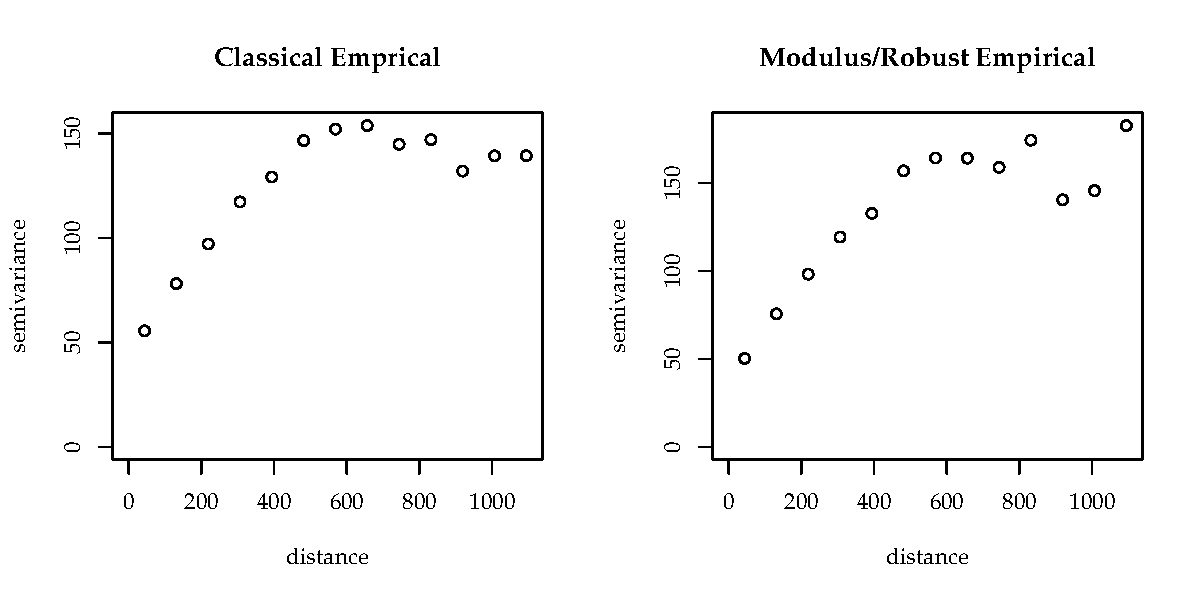
\includegraphics[width=\maxwidth]{figure/emp_var-1} 

}



\end{knitrout}









\section{Selenium Data}



\begin{knitrout}\footnotesize
\definecolor{shadecolor}{rgb}{0.969, 0.969, 0.969}\color{fgcolor}\begin{kframe}


{\ttfamily\noindent\bfseries\color{errorcolor}{Error in array(x, c(length(x), 1L), if (!is.null(names(x))) list(names(x), : 'data' must be of a vector type, was 'NULL'}}\begin{verbatim}
variog: computing omnidirectional variogram
\end{verbatim}
\end{kframe}

{\centering 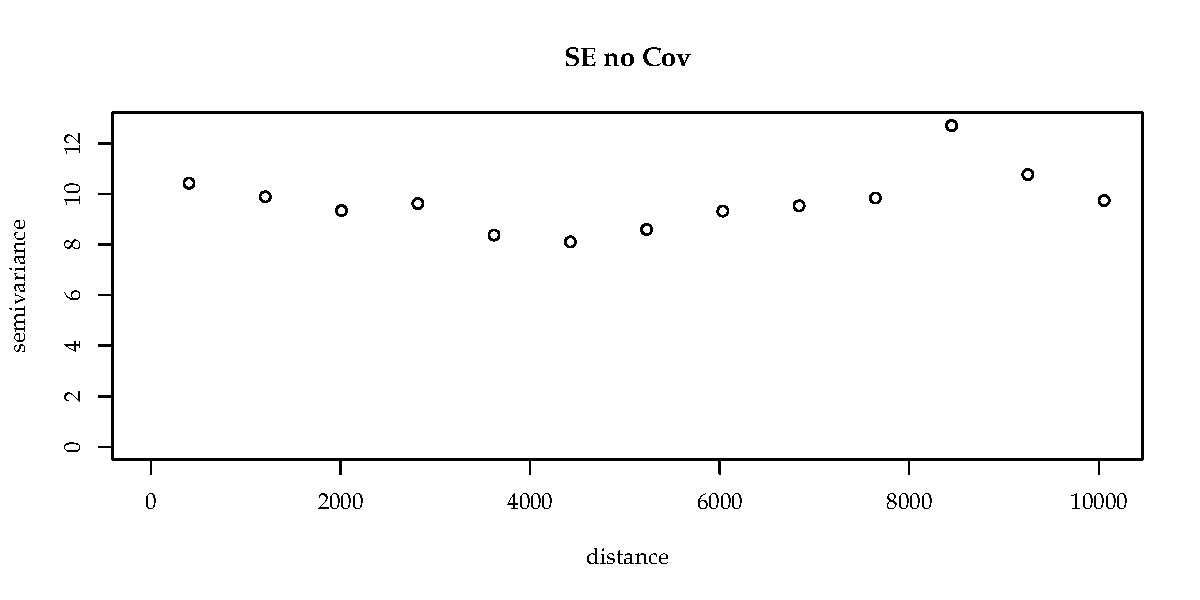
\includegraphics[width=\maxwidth]{figure/sims_se-1} 

}


\begin{kframe}\begin{verbatim}
variog: computing omnidirectional variogram
\end{verbatim}
\end{kframe}

{\centering 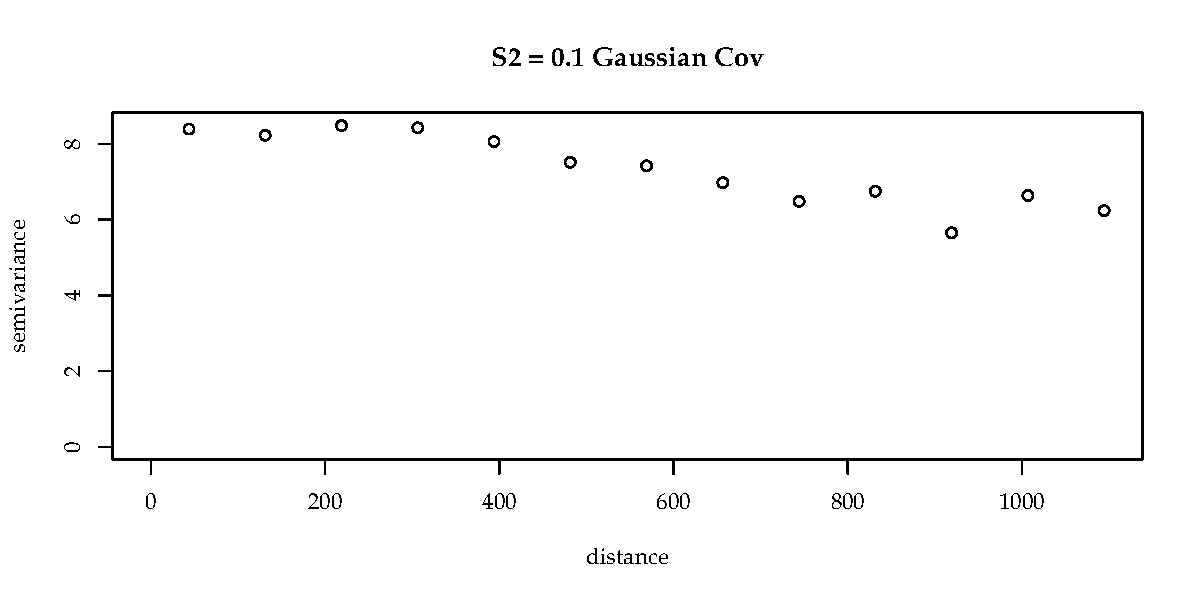
\includegraphics[width=\maxwidth]{figure/sims_se-2} 

}


\begin{kframe}\begin{verbatim}
variog: computing omnidirectional variogram
\end{verbatim}
\end{kframe}

{\centering 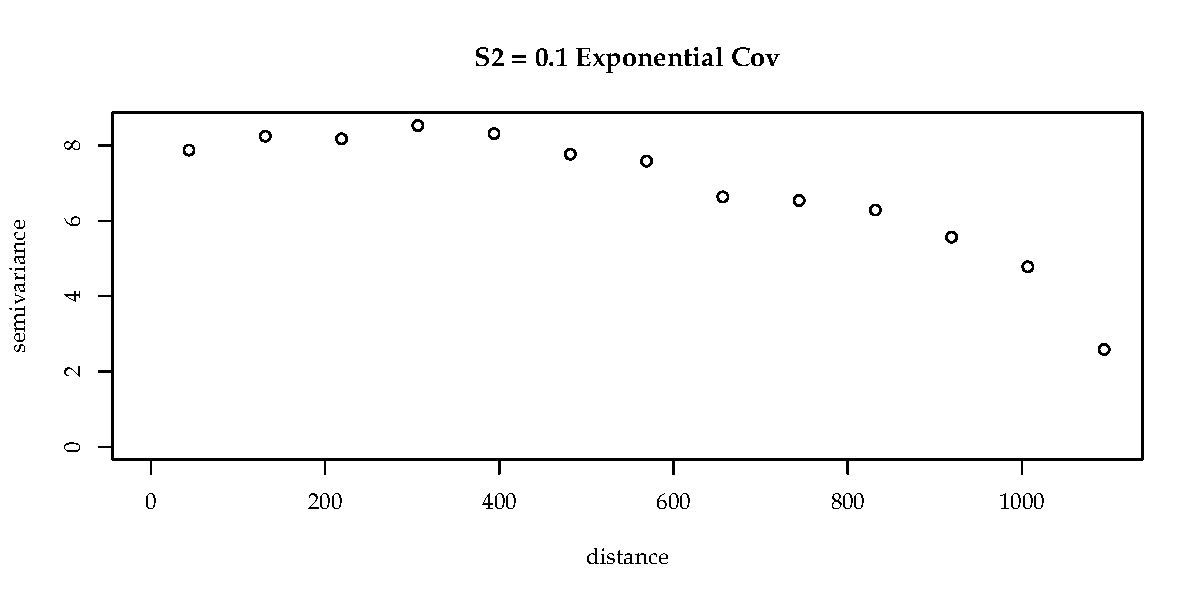
\includegraphics[width=\maxwidth]{figure/sims_se-3} 

}


\begin{kframe}

{\ttfamily\noindent\bfseries\color{errorcolor}{Error in variog(data = Z, coords = ca\$coords): object 'Z' not found}}\begin{verbatim}
variog: computing omnidirectional variogram
variog: computing omnidirectional variogram
\end{verbatim}
\end{kframe}

{\centering 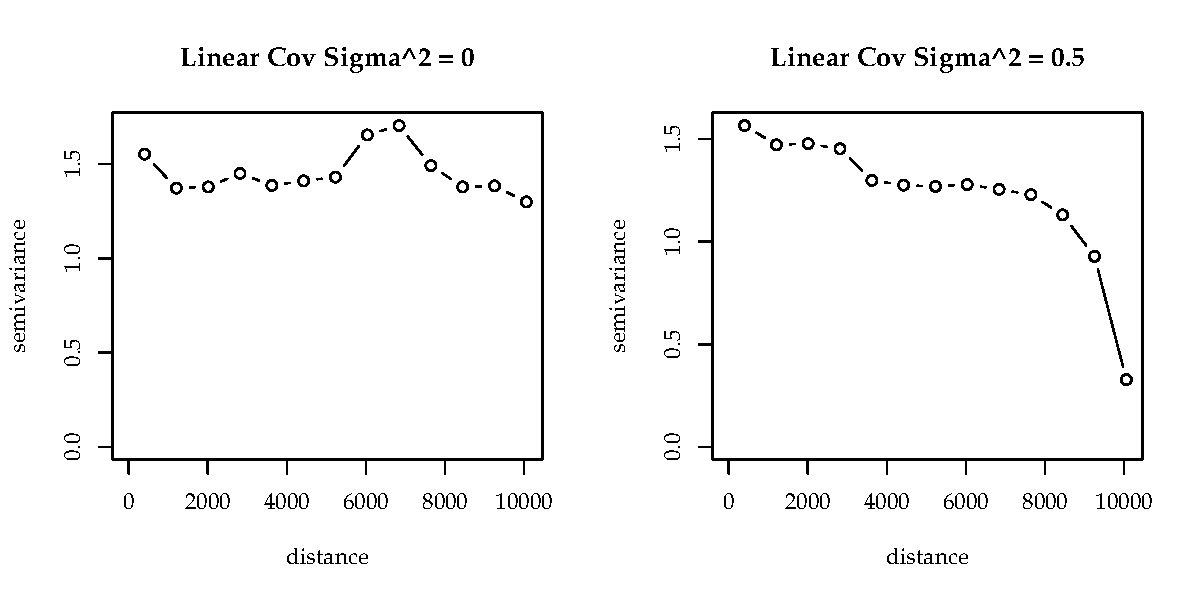
\includegraphics[width=\maxwidth]{figure/sims_se-4} 

}


\begin{kframe}\begin{verbatim}
variog: computing omnidirectional variogram
variog: computing omnidirectional variogram
\end{verbatim}
\end{kframe}

{\centering 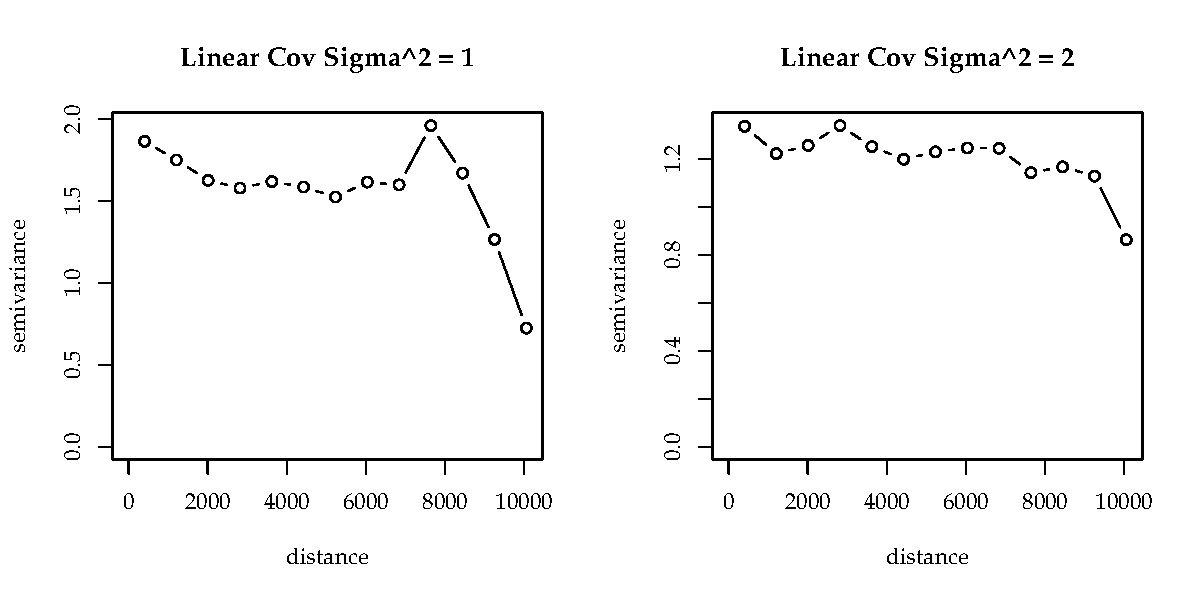
\includegraphics[width=\maxwidth]{figure/sims_se-5} 

}


\begin{kframe}\begin{verbatim}
variog: computing omnidirectional variogram
\end{verbatim}
\end{kframe}

{\centering 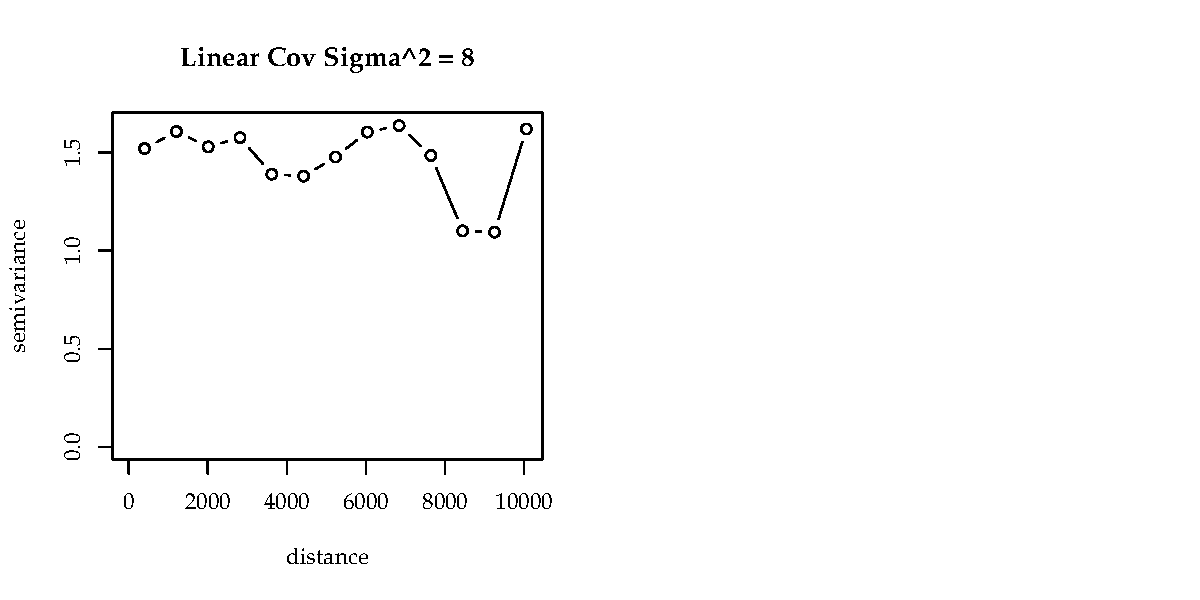
\includegraphics[width=\maxwidth]{figure/sims_se-6} 

}


\begin{kframe}\begin{verbatim}
variog: computing omnidirectional variogram
variog: computing omnidirectional variogram
\end{verbatim}
\end{kframe}

{\centering 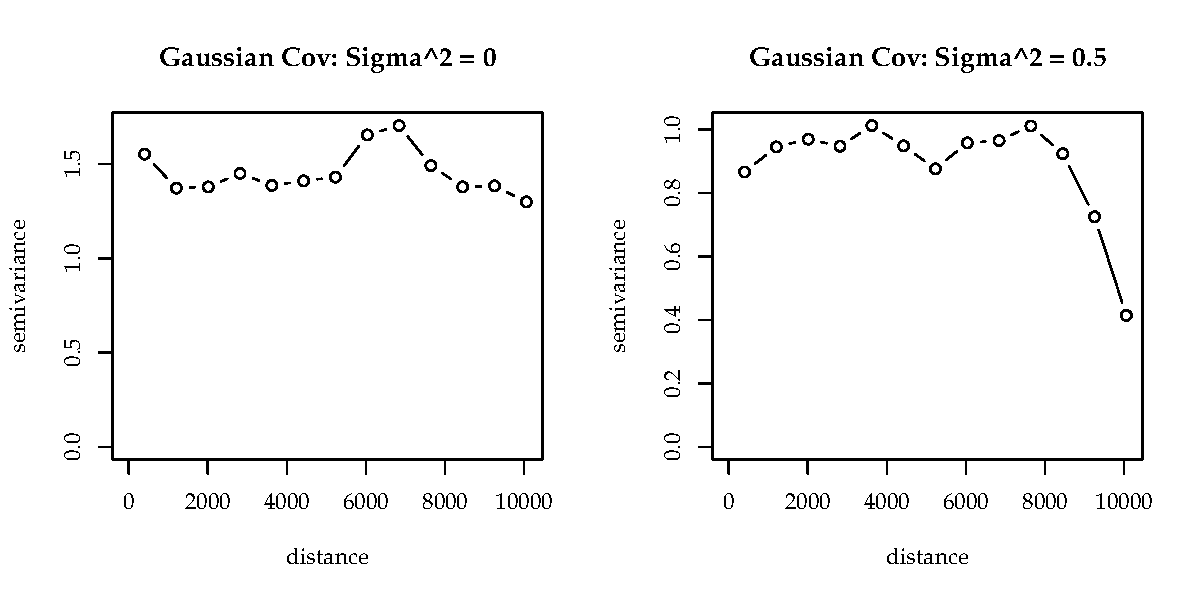
\includegraphics[width=\maxwidth]{figure/sims_se-7} 

}


\begin{kframe}\begin{verbatim}
variog: computing omnidirectional variogram
\end{verbatim}
\end{kframe}

{\centering 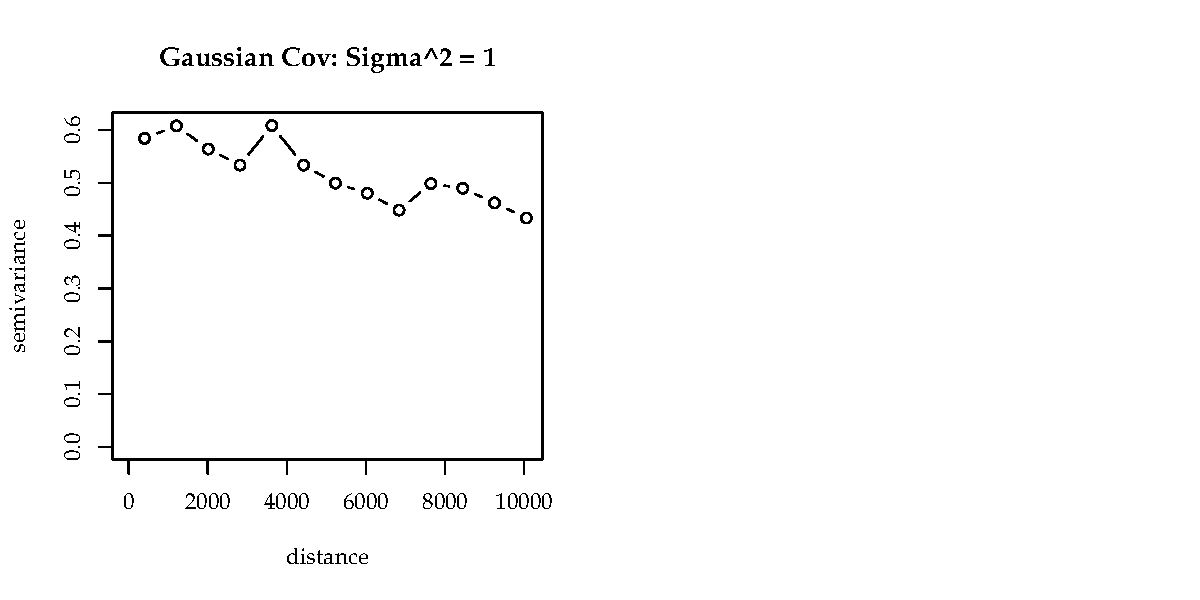
\includegraphics[width=\maxwidth]{figure/sims_se-8} 

}


\begin{kframe}\begin{verbatim}
variog: computing omnidirectional variogram
variog: computing omnidirectional variogram
\end{verbatim}
\end{kframe}

{\centering 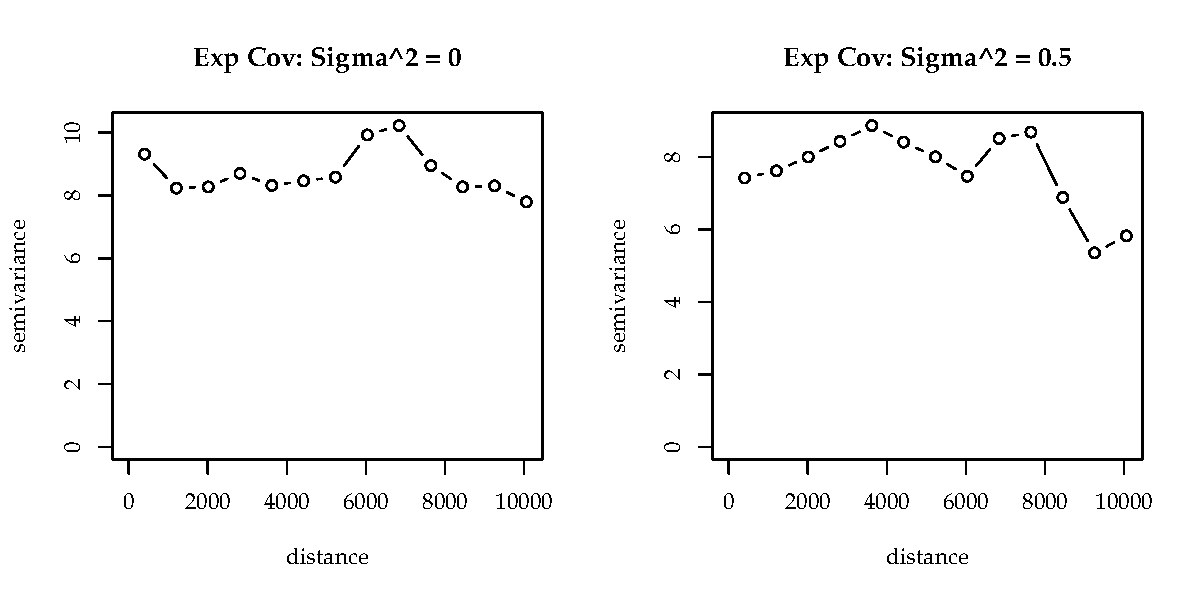
\includegraphics[width=\maxwidth]{figure/sims_se-9} 

}


\begin{kframe}\begin{verbatim}
variog: computing omnidirectional variogram
variog: computing omnidirectional variogram
\end{verbatim}
\end{kframe}

{\centering 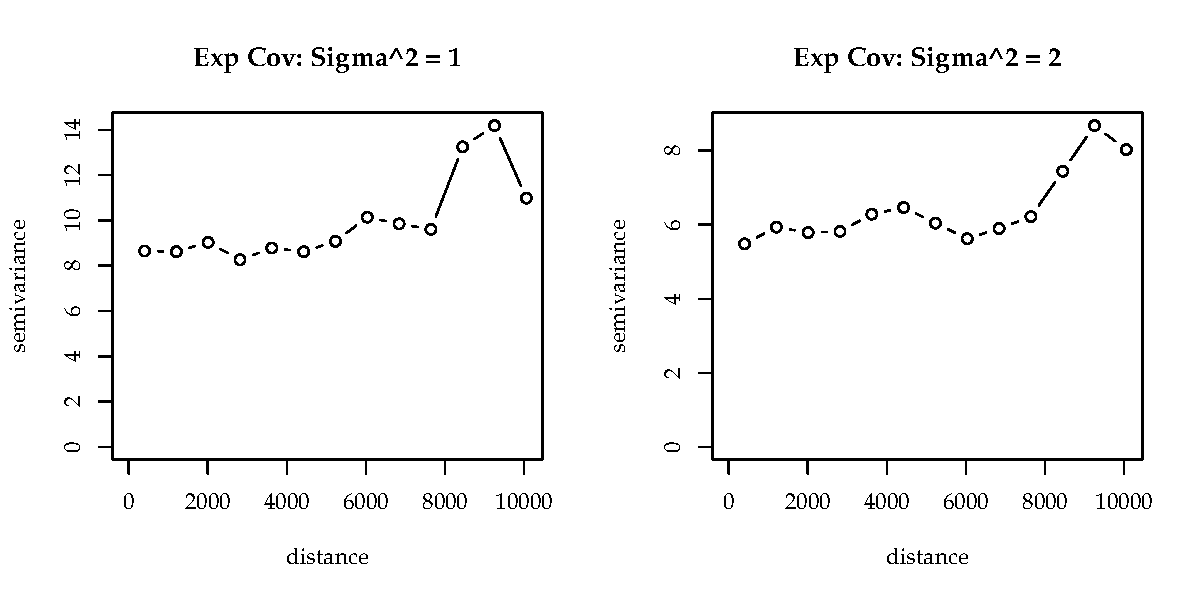
\includegraphics[width=\maxwidth]{figure/sims_se-10} 

}


\begin{kframe}\begin{verbatim}
variog: computing omnidirectional variogram
variog: computing omnidirectional variogram
\end{verbatim}
\end{kframe}

{\centering 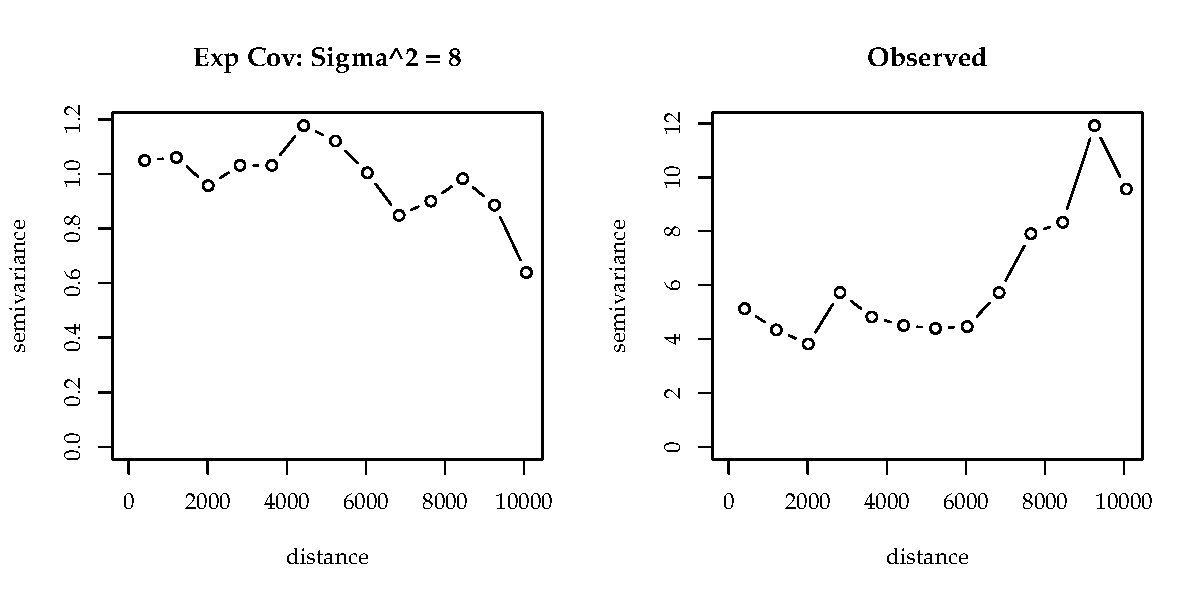
\includegraphics[width=\maxwidth]{figure/sims_se-11} 

}


\begin{kframe}\begin{verbatim}
variog: computing variogram for direction = 0 degrees (0 radians)
        tolerance angle = 22.5 degrees (0.393 radians)
variog: computing variogram for direction = 45 degrees (0.785 radians)
        tolerance angle = 22.5 degrees (0.393 radians)
variog: computing variogram for direction = 90 degrees (1.571 radians)
        tolerance angle = 22.5 degrees (0.393 radians)
variog: computing variogram for direction = 135 degrees (2.356 radians)
        tolerance angle = 22.5 degrees (0.393 radians)
variog: computing omnidirectional variogram
\end{verbatim}
\end{kframe}

{\centering 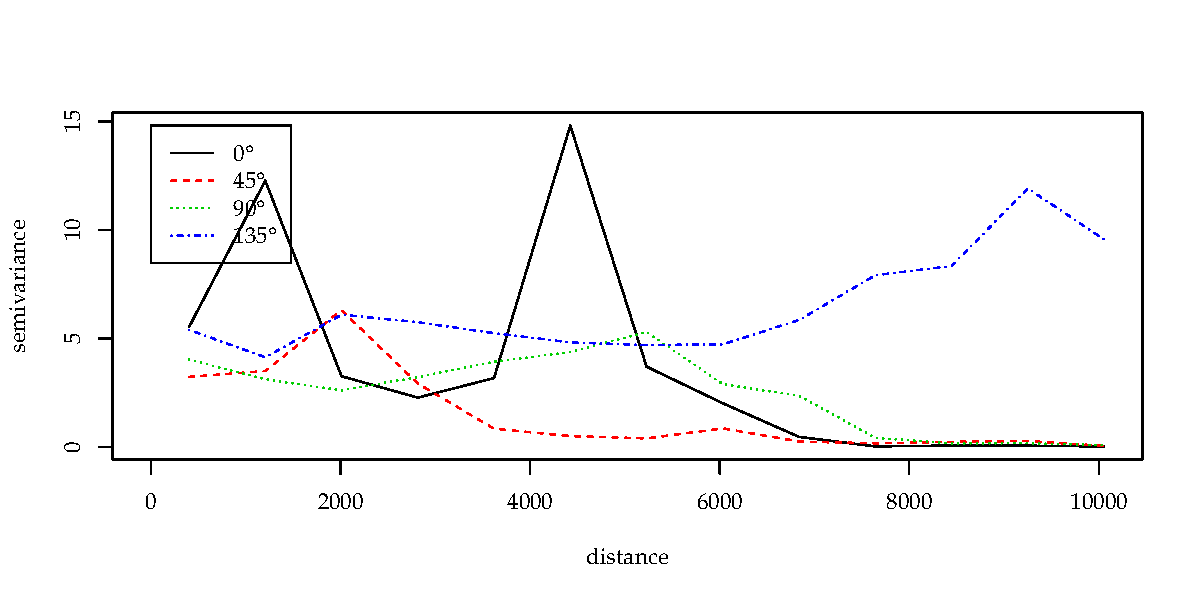
\includegraphics[width=\maxwidth]{figure/sims_se-12} 

}


\begin{kframe}\begin{verbatim}
variog: computing omnidirectional variogram
\end{verbatim}
\end{kframe}

{\centering 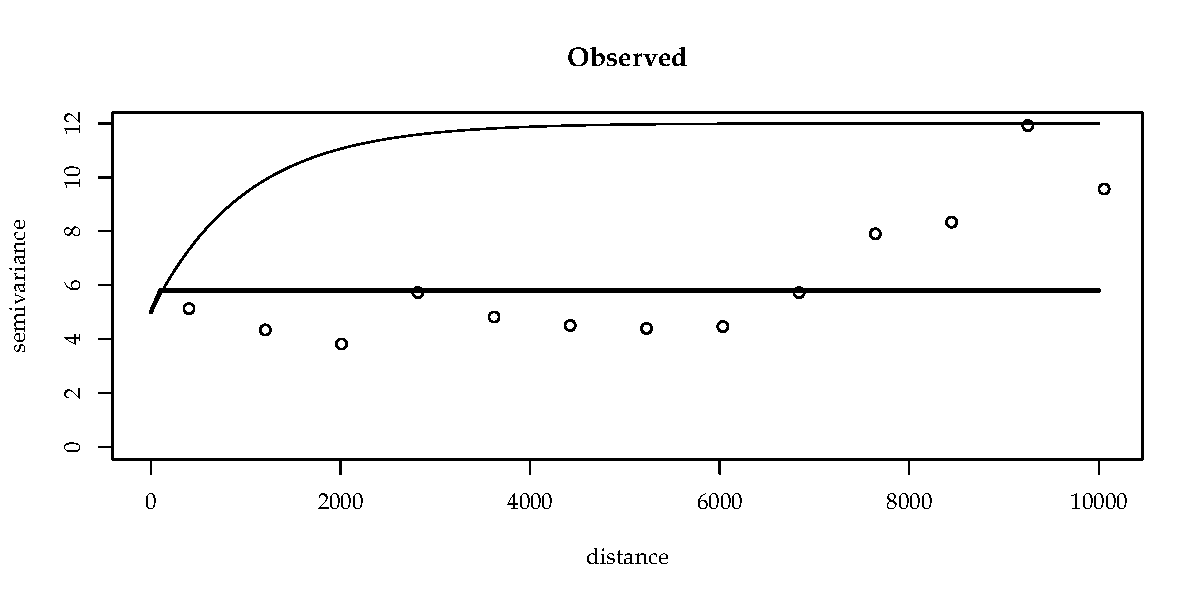
\includegraphics[width=\maxwidth]{figure/sims_se-13} 

}



\end{knitrout}


\end{document}



